% Number 30
% Algebra
% Number of coins - algebra problem
% MIT Physics for Teachers LON-CAPA

% Watermark
\AddToShipoutPicture*{\BackgroundPic}

\addtocounter {ProbNum} {1}

%\begin{floatingfigure}[r]{.2\textwidth}
%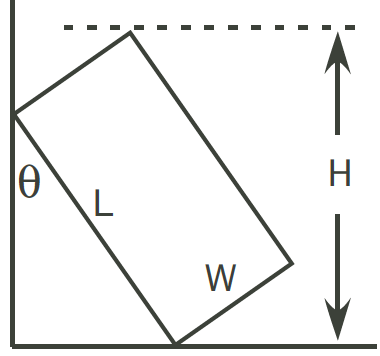
\includegraphics[scale=1]{/Users/jgates/desktop/latex/pics/leaningbox.png}
%\end{floatingfigure}
 
{\bf \Large{\arabic{ProbNum}}} Britney has 25 coins, all nickels (5 cents) and dimes (10 cents). If the nickels were changed to quarters (25 cents) and the dimes changed to nickels, the total value of the coins would remain unchanged. 

\bigskip

\indent How many nickels and how many dimes does she have? 

\vfill

\newpage
